\documentclass[crop,tikz]{standalone}

\usetikzlibrary{mindmap}

%\setlength\parindent{0pt}
\renewcommand{\footnotesize}{\fontsize{5.5}{6.0}\selectfont}
\renewcommand{\normalsize}{\fontsize{7.5}{11.0}\selectfont}
\begin{document}
	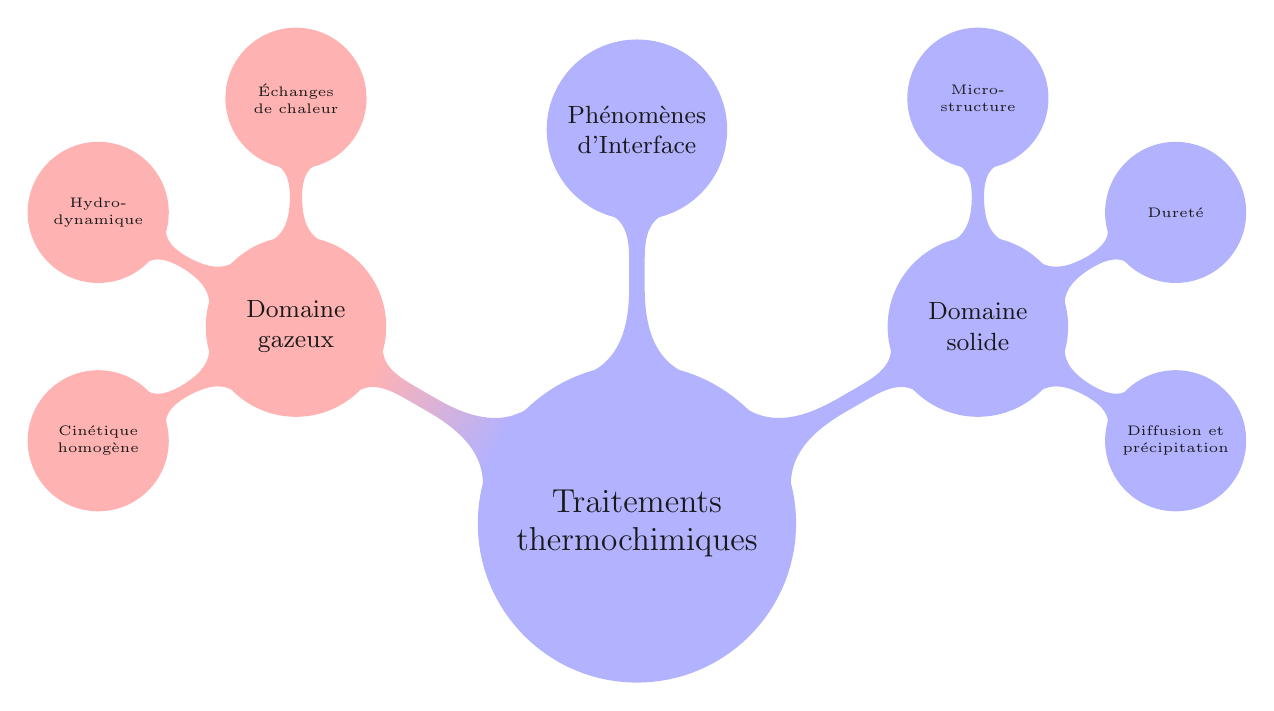
\begin{tikzpicture}
		\path[mindmap,concept color=blue!30,text=black!90]
		node[concept] {Traitements thermochimiques}
		[clockwise from=150]
		child[concept color=red!30] { 
			node[concept] {Domaine gazeux}
			[clockwise from=210]
			child { node[concept] {Cinétique homogène} }
			child { node[concept] {Hydro\-dynamique} }
			child { node[concept] {Échanges\ de\ chaleur} }
		}
		child[concept] {
			node[concept] {Phénomènes d'Interface} 
		}
		child[concept] { 
			node[concept] {Domaine solide}
			[clockwise from=90]
			child { node[concept] {Micro\-structure} }
			child { node[concept] {Dureté} }
			child { node[concept] {Diffusion et précipitation} }
		};
	\end{tikzpicture}
\end{document}